\documentclass{standalone}
\usepackage{tikz}
\usetikzlibrary{patterns, positioning}

\begin{document}
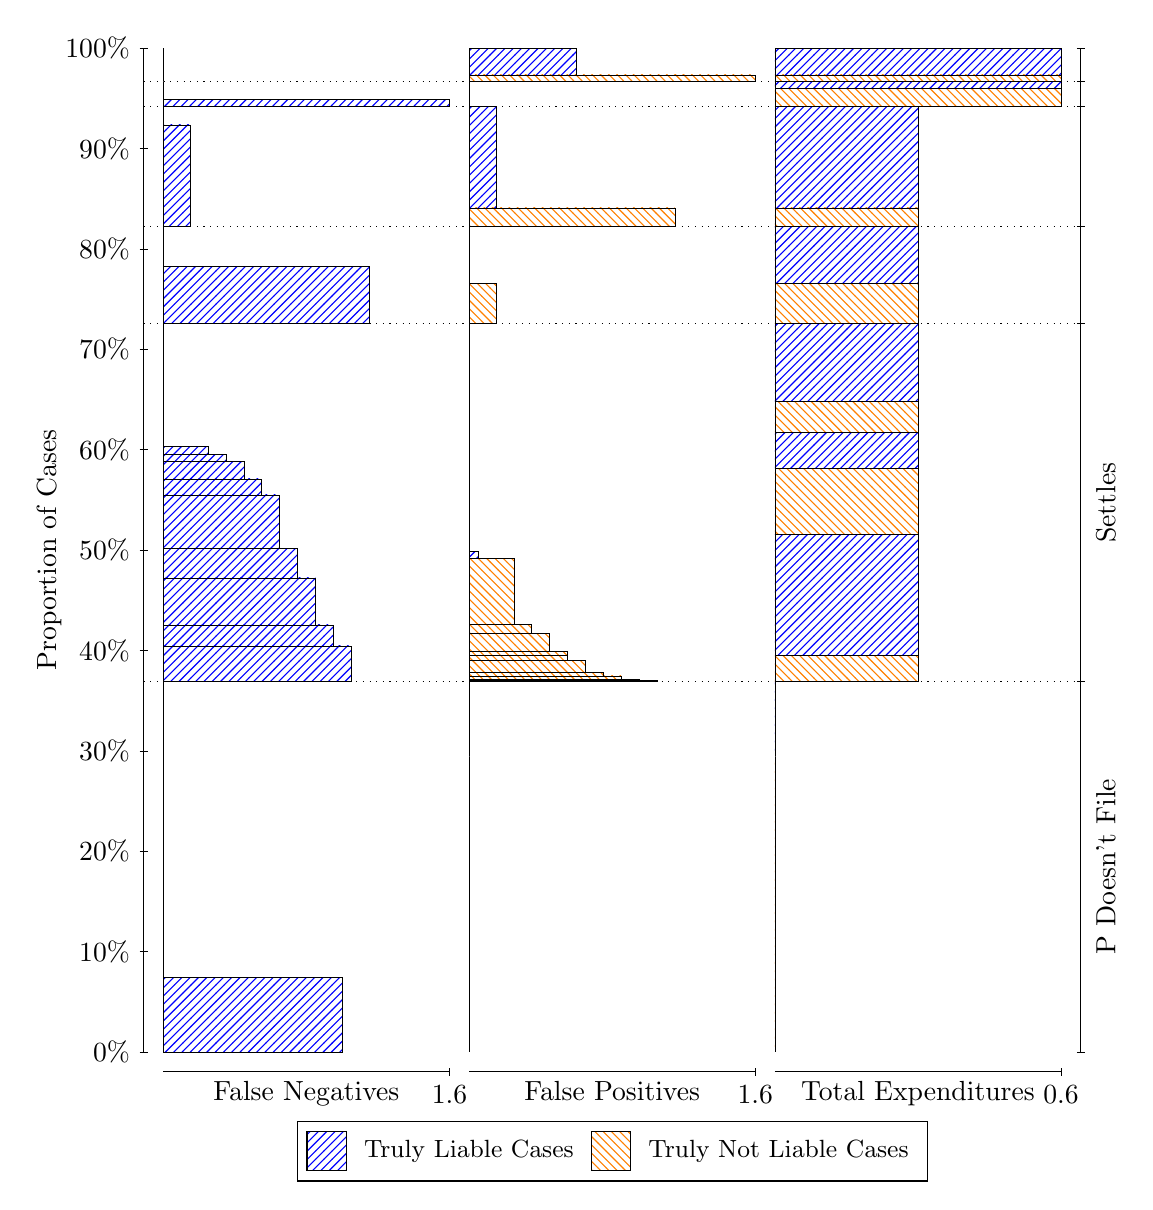
\begin{tikzpicture}
\draw[black, very thin] (1.5,1.75) -- (1.5,14.5);
\node[rotate=90, anchor=center] at (0.3, 8.125) {Proportion of Cases};
\draw[black, very thin] (1.45,1.75) -- (1.55,1.75);
\node[anchor=east] at (1.45, 1.75) {0\%};
\draw[black, very thin] (1.45,3.025) -- (1.55,3.025);
\node[anchor=east] at (1.45, 3.025) {10\%};
\draw[black, very thin] (1.45,4.3) -- (1.55,4.3);
\node[anchor=east] at (1.45, 4.3) {20\%};
\draw[black, very thin] (1.45,5.575) -- (1.55,5.575);
\node[anchor=east] at (1.45, 5.575) {30\%};
\draw[black, very thin] (1.45,6.85) -- (1.55,6.85);
\node[anchor=east] at (1.45, 6.85) {40\%};
\draw[black, very thin] (1.45,8.125) -- (1.55,8.125);
\node[anchor=east] at (1.45, 8.125) {50\%};
\draw[black, very thin] (1.45,9.4) -- (1.55,9.4);
\node[anchor=east] at (1.45, 9.4) {60\%};
\draw[black, very thin] (1.45,10.675) -- (1.55,10.675);
\node[anchor=east] at (1.45, 10.675) {70\%};
\draw[black, very thin] (1.45,11.95) -- (1.55,11.95);
\node[anchor=east] at (1.45, 11.95) {80\%};
\draw[black, very thin] (1.45,13.225) -- (1.55,13.225);
\node[anchor=east] at (1.45, 13.225) {90\%};
\draw[black, very thin] (1.45,14.5) -- (1.55,14.5);
\node[anchor=east] at (1.45, 14.5) {100\%};

\draw[black, very thin] (13.4,1.75) -- (13.4,14.5);
\draw[black, very thin] (13.35,1.75) -- (13.45,1.75);
\node[anchor=west] at (13.35, 1.75) {};
\draw[black, very thin] (13.35,6.452) -- (13.45,6.452);
\node[anchor=west] at (13.35, 6.452) {};
\draw[black, very thin] (13.35,11) -- (13.45,11);
\node[anchor=west] at (13.35, 11) {};
\draw[black, very thin] (13.35,12.235) -- (13.45,12.235);
\node[anchor=west] at (13.35, 12.235) {};
\draw[black, very thin] (13.35,13.76) -- (13.45,13.76);
\node[anchor=west] at (13.35, 13.76) {};
\draw[black, very thin] (13.35,14.075) -- (13.45,14.075);
\node[anchor=west] at (13.35, 14.075) {};
\draw[black, very thin] (13.35,14.5) -- (13.45,14.5);
\node[anchor=west] at (13.35, 14.5) {};

\draw[black, very thin, pattern color=blue, pattern=north east lines] (1.75,1.75) rectangle (4.0208,2.6993);
\draw[black, very thin, pattern color=orange, pattern=north west lines] (1.75,2.6993) rectangle (1.75,6.452);
\draw[black, very thin, pattern color=blue, pattern=north east lines] (1.75,6.452) rectangle (4.1344,6.9085);
\draw[black, very thin, pattern color=blue, pattern=north east lines] (1.75,6.9085) rectangle (3.9073,7.1738);
\draw[black, very thin, pattern color=blue, pattern=north east lines] (1.75,7.1738) rectangle (3.6802,7.7718);
\draw[black, very thin, pattern color=blue, pattern=north east lines] (1.75,7.7718) rectangle (3.4531,8.1415);
\draw[black, very thin, pattern color=blue, pattern=north east lines] (1.75,8.1415) rectangle (3.226,8.8246);
\draw[black, very thin, pattern color=blue, pattern=north east lines] (1.75,8.8246) rectangle (2.999,9.027);
\draw[black, very thin, pattern color=blue, pattern=north east lines] (1.75,9.027) rectangle (2.7719,9.2514);
\draw[black, very thin, pattern color=blue, pattern=north east lines] (1.75,9.2514) rectangle (2.5448,9.3397);
\draw[black, very thin, pattern color=blue, pattern=north east lines] (1.75,9.3397) rectangle (2.3177,9.436);
\draw[black, very thin, pattern color=orange, pattern=north west lines] (1.75,9.436) rectangle (1.75,11);
\draw[black, very thin, pattern color=blue, pattern=north east lines] (1.75,11) rectangle (4.3615,11.727);
\draw[black, very thin, pattern color=orange, pattern=north west lines] (1.75,11.727) rectangle (1.75,12.235);
\draw[black, very thin, pattern color=blue, pattern=north east lines] (1.75,12.235) rectangle (2.0906,13.525);
\draw[black, very thin, pattern color=orange, pattern=north west lines] (1.75,13.525) rectangle (1.75,13.76);
\draw[black, very thin, pattern color=blue, pattern=north east lines] (1.75,13.76) rectangle (5.3833,13.844);
\draw[black, very thin, pattern color=orange, pattern=north west lines] (1.75,13.844) rectangle (1.75,14.075);
\draw[black, very thin, pattern color=orange, pattern=north west lines] (1.75,14.075) rectangle (1.75,14.16);
\draw[black, very thin, pattern color=blue, pattern=north east lines] (1.75,14.16) rectangle (1.75,14.5);
\draw[black, very thin, pattern color=orange, pattern=north west lines] (5.6333,1.75) rectangle (5.6333,5.5027);
\draw[black, very thin, pattern color=blue, pattern=north east lines] (5.6333,5.5027) rectangle (5.6333,6.452);
\draw[black, very thin, pattern color=orange, pattern=north west lines] (5.6333,6.452) rectangle (8.0177,6.468);
\draw[black, very thin, pattern color=orange, pattern=north west lines] (5.6333,6.468) rectangle (7.7906,6.4855);
\draw[black, very thin, pattern color=orange, pattern=north west lines] (5.6333,6.4855) rectangle (7.5635,6.5266);
\draw[black, very thin, pattern color=orange, pattern=north west lines] (5.6333,6.5266) rectangle (7.3365,6.5678);
\draw[black, very thin, pattern color=orange, pattern=north west lines] (5.6333,6.5678) rectangle (7.1094,6.7271);
\draw[black, very thin, pattern color=orange, pattern=north west lines] (5.6333,6.7271) rectangle (6.8823,6.7891);
\draw[black, very thin, pattern color=orange, pattern=north west lines] (5.6333,6.7891) rectangle (6.8823,6.8377);
\draw[black, very thin, pattern color=orange, pattern=north west lines] (5.6333,6.8377) rectangle (6.6552,7.0628);
\draw[black, very thin, pattern color=orange, pattern=north west lines] (5.6333,7.0628) rectangle (6.4281,7.1831);
\draw[black, very thin, pattern color=orange, pattern=north west lines] (5.6333,7.1831) rectangle (6.201,8.0158);
\draw[black, very thin, pattern color=blue, pattern=north east lines] (5.6333,8.0158) rectangle (5.7469,8.1121);
\draw[black, very thin, pattern color=blue, pattern=north east lines] (5.6333,8.1121) rectangle (5.6333,11);
\draw[black, very thin, pattern color=orange, pattern=north west lines] (5.6333,11) rectangle (5.974,11.508);
\draw[black, very thin, pattern color=blue, pattern=north east lines] (5.6333,11.508) rectangle (5.6333,12.235);
\draw[black, very thin, pattern color=orange, pattern=north west lines] (5.6333,12.235) rectangle (8.2448,12.469);
\draw[black, very thin, pattern color=blue, pattern=north east lines] (5.6333,12.469) rectangle (5.974,13.76);
\draw[black, very thin, pattern color=orange, pattern=north west lines] (5.6333,13.76) rectangle (5.6333,13.991);
\draw[black, very thin, pattern color=blue, pattern=north east lines] (5.6333,13.991) rectangle (5.6333,14.075);
\draw[black, very thin, pattern color=orange, pattern=north west lines] (5.6333,14.075) rectangle (9.2667,14.16);
\draw[black, very thin, pattern color=blue, pattern=north east lines] (5.6333,14.16) rectangle (6.9958,14.5);
\draw[black, very thin, pattern color=orange, pattern=north west lines] (9.5167,1.75) rectangle (9.5167,5.5027);
\draw[black, very thin, pattern color=blue, pattern=north east lines] (9.5167,5.5027) rectangle (9.5167,6.452);
\draw[black, very thin, pattern color=orange, pattern=north west lines] (9.5167,6.452) rectangle (11.333,6.7891);
\draw[black, very thin, pattern color=blue, pattern=north east lines] (9.5167,6.7891) rectangle (11.333,8.3257);
\draw[black, very thin, pattern color=orange, pattern=north west lines] (9.5167,8.3257) rectangle (11.333,9.1584);
\draw[black, very thin, pattern color=blue, pattern=north east lines] (9.5167,9.1584) rectangle (11.333,9.6149);
\draw[black, very thin, pattern color=orange, pattern=north west lines] (9.5167,9.6149) rectangle (11.333,10.009);
\draw[black, very thin, pattern color=blue, pattern=north east lines] (9.5167,10.009) rectangle (11.333,11);
\draw[black, very thin, pattern color=orange, pattern=north west lines] (9.5167,11) rectangle (11.333,11.508);
\draw[black, very thin, pattern color=blue, pattern=north east lines] (9.5167,11.508) rectangle (11.333,12.235);
\draw[black, very thin, pattern color=orange, pattern=north west lines] (9.5167,12.235) rectangle (11.333,12.469);
\draw[black, very thin, pattern color=blue, pattern=north east lines] (9.5167,12.469) rectangle (11.333,13.76);
\draw[black, very thin, pattern color=orange, pattern=north west lines] (9.5167,13.76) rectangle (13.15,13.991);
\draw[black, very thin, pattern color=blue, pattern=north east lines] (9.5167,13.991) rectangle (13.15,14.075);
\draw[black, very thin, pattern color=orange, pattern=north west lines] (9.5167,14.075) rectangle (13.15,14.16);
\draw[black, very thin, pattern color=blue, pattern=north east lines] (9.5167,14.16) rectangle (13.15,14.5);
\draw[black, dotted] (1.5,6.452) -- (13.4,6.452);
\draw[black, dotted] (1.5,11) -- (13.4,11);
\draw[black, dotted] (1.5,12.235) -- (13.4,12.235);
\draw[black, dotted] (1.5,13.76) -- (13.4,13.76);
\draw[black, dotted] (1.5,14.075) -- (13.4,14.075);
\draw[black, very thin] (1.75,1.5) -- (5.3833,1.5);
\node[anchor=north] at (3.5667, 1.5) {False Negatives};
\draw[black, very thin] (5.3833,1.45) -- (5.3833,1.55);
\node[anchor=north] at (5.3833, 1.45) {1.6};

\draw[black, very thin] (5.6333,1.5) -- (9.2667,1.5);
\node[anchor=north] at (7.45, 1.5) {False Positives};
\draw[black, very thin] (9.2667,1.45) -- (9.2667,1.55);
\node[anchor=north] at (9.2667, 1.45) {1.6};

\draw[black, very thin] (9.5167,1.5) -- (13.15,1.5);
\node[anchor=north] at (11.333, 1.5) {Total Expenditures};
\draw[black, very thin] (13.15,1.45) -- (13.15,1.55);
\node[anchor=north] at (13.15, 1.45) {0.6};

\node[black, centered, rotate=90] at (13.72, 4.101) {P Doesn't File};
\node[black, centered, rotate=90] at (13.72, 8.7259) {Settles};





\draw (7.449999999999999,1.5) node[draw=none] (baseCoordinate) {};
\begin{scope}[align=center]
        \matrix[scale=0.5, draw=black, below=0.5cm of baseCoordinate, nodes={draw}, column sep=0.1cm]{
            \node[rectangle, draw, minimum width=0.5cm, minimum height=0.5cm, pattern=north east lines, pattern color=blue] {}; &
            \node[draw=none, font=\small] (B) {Truly Liable Cases}; &
            \node[rectangle, draw, minimum width=0.5cm, minimum height=0.5cm, pattern=north west lines, pattern color=orange] {}; &
            \node[draw=none, font=\small] (B) {Truly Not Liable Cases}; \\
            };
\end{scope}

\end{tikzpicture}
\end{document}